% Fixes conflict of the packages tkiz and xcolor about the options usenames and
% dvipsnames which we want to pass to xcolor.
\PassOptionsToPackage{usenames,dvipsnames,table}{xcolor}

\documentclass[12pt]{beamer}

\usepackage{tikz}
\usetikzlibrary{positioning,calc,arrows.meta,automata,shadows}
%\usepackage{mathtools}
%\usepackage{amssymb}
%\usepackage{xcolor}
%\usepackage[noend]{algpseudocode}

% Allow literal typing of ä, ö, ü, etc.
\usepackage[utf8]{inputenc}

% Allows to set background colour of table cell
\usepackage[table]{xcolor}

% For not adding frames after \appendix to total number of slides
\usepackage{appendixnumberbeamer}

% Table column type m{...}
\usepackage{array}

% Smart filename extension recognition (allow dots in file names)
\usepackage{grffile}

% Tabstops like in Word (\tabto{4cm})
\usepackage{tabto}

% Allows to set opacity with \transparent
\usepackage{transparent}


% URL style (related to package 'hyperref')
\renewcommand\UrlFont{\color{red}}

%------------------------------------------------------------------------------%
% LaTeX Beamer customisation
%------------------------------------------------------------------------------%
\usetheme{Madrid}

% Turn off the grey navigation symbols at the bottom
\setbeamertemplate{navigation symbols}{}

% Turn off navigation header
%\setbeamertemplate{headline}{}

% Font size for footnotes
\setbeamerfont{footnote}{size=\scriptsize}

% Serif font for math mode
\usefonttheme[onlymath]{serif}

% Make covered text (\pause) transparent instead of hidden
\setbeamercovered{transparent}

% More table cell spacing (standard Latex thing)
%\renewcommand{\arraystretch}{1.5}
%\renewcommand{\tabcolsep}{0.2cm}

% Use a number for every bib entry in the bibliography, instead of small images
\setbeamertemplate{bibliography item}[text]

% Font sizes (\fontsize{size}{lineheight})
%\setbeamerfont{frametitle}{size={\fontsize{20}{25}}}
\setbeamerfont{author}{size={\fontsize{10}{10}}}
\setbeamerfont{institute}{size={\fontsize{10}{10}}}
\setbeamerfont{date}{size={\fontsize{10}{10}}}

% Make outline font, bold and black
\setbeamerfont{section in toc}{series=\bfseries}
\setbeamercolor{section in toc}{fg=black}

% Replace the ugly balls in the outline with normal numbers
\setbeamertemplate{sections/subsections in toc}[sections numbered]

% Normal numbers in 'enumerate' (instead balls)
\setbeamertemplate{enumerate items}[default]

% Set itemize items (there is [ball], [circle], [square], [triangle])
\setbeamertemplate{itemize items}[circle]
\setbeamertemplate{itemize subitem}[triangle]

% Redefinition of the footline. Found at
% http://tex.stackexchange.com/questions/66995/modify-footer-of-slides
% Note that if the indicated '%' signs are removed, there appear gaps. The
% answer seems to be that the '%' comment causes LaTeX to ignore the '\n' at
% the end of the line, which otherwise it might replace with a whitespace. This
% whitespace might be the cause for a gap.
% "author in head/foot", etc. seem to be defined colors.
% dw-25.05.2013
\makeatother
\setbeamertemplate{footline}
{
  \hbox{% If this '%' sign is deleted, there's a gap before 1st box
    \begin{beamercolorbox}[wd=0.333\paperwidth,ht=2.25ex,dp=1ex,center]{author in head/foot}
      \insertshortauthor
    \end{beamercolorbox}% If '%' deleted, gap between 1st and 2nd box
    \begin{beamercolorbox}[wd=0.333\paperwidth,ht=2.25ex,dp=1ex,center]{title in head/foot}
      \insertshortdate
    \end{beamercolorbox}% If '%' deleted, gap between 2nd and 3rd box
    \begin{beamercolorbox}[wd=.333\paperwidth,ht=2.25ex,dp=1ex,center]{date in head/foot}
        \insertframenumber{} / \inserttotalframenumber
    \end{beamercolorbox}
  }
}
\makeatletter

% Environment for disabling header and footer
\makeatletter
    \newenvironment{blank}{
        \setbeamertemplate{headline}{}
        \def\beamer@entrycode{\vspace*{-\headheight}}
        \setbeamertemplate{footline}{}
    }{}
\makeatother

%------------------------------------------------------------------------------%
% TikZ customisation
%------------------------------------------------------------------------------%

\tikzset{
  >=stealth,
  my state/.style={
    draw,
    minimum height=1.5em,
    minimum width=1.5em,
    inner sep=0.5mm,
    rounded corners=1mm,
    rectangle
  },
  my accepting/.style={
    double,
    double distance=0.8pt,
    outer sep=0.7pt,
  },
  my automaton/.style={
    every state/.style={my state},
    accepting/.style={my accepting},
    initial text=,
    every loop/.style={min distance=6mm,looseness=7},
    my above/.style={out=115,in=65},
    my below/.style={out=245,in=295},
    my right/.style={out=25,in=335},
    node distance=0.75cm
  }
}

% Color of definition blocks
\setbeamercolor{block title}{fg=black,bg=white!75!black}

%------------------------------------------------------------------------------%
% New commands
%------------------------------------------------------------------------------%
% Shorthand commands
\newcommand{\fat}[1]{\textbf{#1}}
\newcommand{\ita}[1]{\textit{#1}}

% Formatting of a slice containing only the table of contents
\newcommand{\tocstyle}[1]{
\Large
\vspace{0.25cm}
\hspace{0.5cm}
\parbox[top][0.66\textheight][c]{0.66\textwidth}{#1}}

% Active cell in the IG-IM-EG-EM matrix
\newcommand{\activecell}[1]{\cellcolor{red}\color{white}{#1}}

% Michel 4
\newcommand{\Michel}{
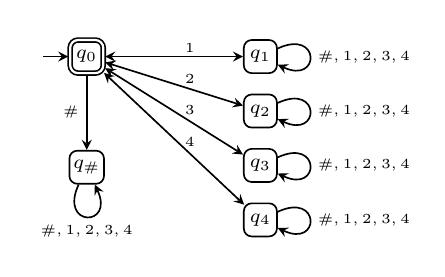
\begin{tikzpicture}[my automaton,semithick]
\scriptsize
% Initial node and #-node
\node[state,initial,accepting] (0)               {$q_0$};
\node[state,yshift=-0.2cm]                   (x) [below=of 0]  {$q_\#$};
\draw[->] (0) edge node[left] {\tiny\#} (x);
\draw[->] (x) edge[my below,loop] node[below] {\tiny $\#,1,2,3,4$} ();
% Node 1
\node[state,xshift=1cm]        (1) [right=of 0]  {$q_1$};
\draw[<->] (0) edge node[above,xshift=2mm,yshift=-0.5mm] {\tiny $1$} (1);
\draw[->] (1) edge[my right,loop] node[right] {\tiny $\#,1,2,3,4$} ();
% Node 2
\node[state,yshift=0.5cm]      (2) [below=of 1]  {$q_2$};
\draw[<->] (0) edge node[above,xshift=2mm,yshift=-1mm] {\tiny $2$} (2);
\draw[->] (2) edge[my right,loop] node[right] {\tiny $\#,1,2,3,4$} ();
% Node 3
\node[state,yshift=0.5cm]      (3) [below=of 2]  {$q_3$};
\draw[<->] (0) edge node[above,xshift=2mm,yshift=-1.5mm] {\tiny $3$} (3);
\draw[->] (3) edge[my right,loop] node[right] {\tiny $\#,1,2,3,4$} ();
% Node 4
\node[state,yshift=0.5cm]      (4) [below=of 3]  {$q_4$};
\draw[<->,shorten >=-0.2mm,shorten <=-0.2mm] (0) edge node[above,xshift=2mm,yshift=-2mm] {\tiny $4$} (4);
\draw[->] (4) edge[my right,loop] node[right] {\tiny $\#,1,2,3,4$} ();
\end{tikzpicture}
}

% Directories of figures for result section
\newcommand{\igo}{../results/figures/internal/goal}
\newcommand{\ego}{../results/figures/external/goal}
\newcommand{\imi}{../results/figures/internal/michel}
\newcommand{\emi}{../results/figures/external/michel}

% Dash as itemize symbol
\newcommand{\myitem}{--\hspace*{\labelsep}}

% Listings of constructions in all test scenarios
\newcommand{\igol}{
\begin{tabular}{l}
\myitem Fribourg \\
\myitem Fribourg+R2C \\
\myitem Fribourg+R2C+C \\
\myitem Fribourg+M1 \\
\myitem Fribourg+M1+R2C \\
\myitem Fribourg+M1+R2C+C \\
\myitem Fribourg+M1+M2 \\
\myitem Fribourg+R \\
\end{tabular}}

\newcommand{\imil}{
\begin{tabular}{l}
\myitem Fribourg \\
\myitem Fribourg+R2C \\
\myitem Fribourg+M1 \\
\myitem Fribourg+M1+M2 \\
\myitem Fribourg+M1+M2+R2C \\
\myitem Fribourg+R \\
\end{tabular}}

\newcommand{\egol}{
\begin{tabular}{l}
\myitem Piterman+EQ+RO \\
\myitem Rank+TR+RO \\
\myitem Slice+P+RO+MADJ+EG \\
\myitem Fribourg+M1+R2C \\
\end{tabular}}

\newcommand{\emil}{
\begin{tabular}{l}
\myitem Piterman+EQ+RO \\
\myitem Rank+TR+RO \\
\myitem Slice+P+RO+MADJ+EG \\
\myitem Fribourg+M1+M2+R2C \\
\end{tabular}}

%------------------------------------------------------------------------------%
% Title information
%------------------------------------------------------------------------------%
\title{Empirical Performance Investigation of a Büchi Complementation Construction}
\subtitle{Master's Thesis Presentation} 
\author{Daniel Weibel}
\date{19 August 2015}
\institute{Foundations of Dependable Systems Group\\Department of Informatics\\University of Fribourg\\\texttt{daniel.weibel@unifr.ch}}
% Centered graphics exclusively on the title page
\titlegraphic{\includegraphics[width=6cm]{figures/unifr_logo.pdf}}

\begin{document}

%------------------------------------------------------------------------------%
% Title slide
%------------------------------------------------------------------------------%
{\setbeamertemplate{footline}{}  % Turn off footer on title slice
\begin{frame}
\titlepage
\end{frame}}

%------------------------------------------------------------------------------%
% Outline slide
%------------------------------------------------------------------------------%
\begin{frame}{Outline}
\tocstyle{\tableofcontents}
\end{frame}

\section{Introduction}
%------------------------------------------------------------------------------%
% Frame
%------------------------------------------------------------------------------%
\begin{frame}{Basics}
\begin{block}{Büchi automata}
{\hfill
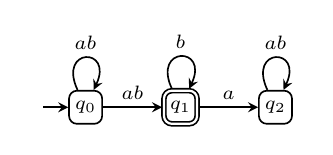
\begin{tikzpicture}[my automaton,semithick]
\scriptsize
\node[state,initial]              (0) {$q_0$};
\node[state,accepting,right=of 0] (1) {$q_1$};
\node[state,,right=of 1]          (2) {$q_2$};
\path[->] (0) edge[my above,loop] node[above] {$ab$} ()
          (0) edge                node[above] {$ab$} (1)
          (1) edge[my above,loop] node[above] {$b$}  ()
          (1) edge                node[above] {$a$}  (2)
          (2) edge[my above,loop] node[above] {$ab$} ();
\end{tikzpicture}\hfill}
\begin{itemize}
  \item Finite state automata running on infinite words ($\omega$-words) $\in \Sigma^\omega$
  \item A word is accepted if it has an accepting run
  \item A run is accepting if it visits an accepting state infinitely often
\end{itemize}
\end{block}
\pause
\begin{block}{Büchi complementation}
The complement of a Büchi automaton $A$ is another Büchi automaton $B$, such that:
\begin{quote}
\ita{$B$ accepts a word if and only if it is not accepted by $A$}
\end{quote}
\end{block}
\end{frame}

%------------------------------------------------------------------------------%
% Frame
%------------------------------------------------------------------------------%
\begin{frame}{State Complexity of Büchi Complementation}
\centering
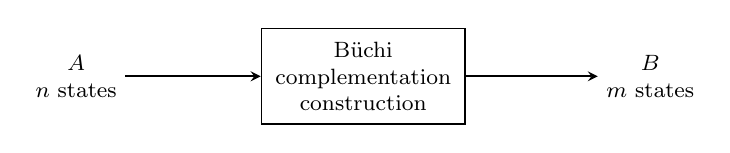
\begin{tikzpicture}[c/.style={align=center},semithick]
\footnotesize
\node (a) [c]                              {$A$\\$n$ states};
\node (b) [c,node distance=6cm,right=of a] {$B$\\$m$ states};
\node (c) at ($(a)!0.5!(b)$) [c,draw,inner sep=5pt]{Büchi\\complementation\\construction};
\draw[->] (a.east) to (c.west);
\draw[->] (c.east) to (b.west);
\end{tikzpicture}
\begin{itemize}
\item State complexity: $m$ in relation to $n$
  \begin{itemize}
  \item Size of complement in relation to size of input automaton
  \end{itemize}
\pause
\item Also known as \ita{state growth}, \ita{state blow-up}, or \ita{state explosion}
\pause
\item Can be \fat{very high}
\item Inhibits the application of Büchi complemetation in practice
  \begin{itemize}
  \item E.g. in automata-theoretic model checking
  \end{itemize}
\pause
\item The lower the state complexity, the higher the performance of the construction
\item Importance to investigate the state complexity of Büchi complementation constructions (see next slides)
\end{itemize}
\end{frame}

%------------------------------------------------------------------------------%
% Frame
%------------------------------------------------------------------------------%
\def\sep{5pt}
\begin{frame}{Worst-Case State Complexity}
\begin{itemize} \itemsep\sep
\item Every construction has a specific worst-case state complexity
\item Maximum number of states that a construction can produce
\pause
\item Examples:
\end{itemize}
\centering
{\footnotesize
\renewcommand{\arraystretch}{1.4}
\renewcommand{\tabcolsep}{0.4cm}
\begin{tabular}{p{3cm}p{2.4cm}p{2.1cm}}
\hline 
Complementation construction & Worst-case state complexity & Example value with $n = 15$ \\
\hline
\cite{buchi1960decision} & $2^{2^{O\left(n\right)}}$ & $1.4 \times 10^{9,864}$ \\
\cite{2007_piterman} & $O(n^{2n})$ & $1.9 \times 10^{35}$ \\
\cite{vardi2007automata} & $O((3n)^n)$ & $6.3 \times 10^{24}$ \\
\cite{schewe2009buchi} & $O((0.76n)^n)$ & $7.1 \times 10^{15}$ \\
\hline
\end{tabular}}
\vspace{\sep}\vspace{2pt}
\begin{itemize}
\pause  
\item Often used to assess the performance or efficiency of a construction, but$\dots$
\end{itemize}
\end{frame}


%------------------------------------------------------------------------------%
% Frame
%------------------------------------------------------------------------------%
\begin{frame}{Empirical Way to Investigate Performance}
\begin{itemize}
\item Worst-case state complexity reflects only a \fat{small} aspect of the state complexity of a construction
\pause
\item From a practical point of view, we are interested in the performance of a construction on \fat{concrete} automata
  \begin{itemize}
  \item E.g. how does the construction perform on ``typical'' automata with 15 states?
  \end{itemize}
\pause
\item Such insights can be gained by \fat{empirical} investigations
\item Empirical performance investigation:
  \begin{enumerate}
  \item[\fat{1.}] \fat{Implement construction}
  \item[\fat{2.}] \fat{Run the implementation on test automata}
  \item[\fat{3.}] \fat{Analyse generated complements}
  \end{enumerate}
\pause
\item Aim of this thesis:
  \begin{itemize}
  \item Empirically investigate the performance of the \fat{Fribourg construction} (see next slide)
  \end{itemize}
\end{itemize}
\end{frame}


%------------------------------------------------------------------------------%
% Frame
%------------------------------------------------------------------------------%
\begin{frame}{The Fribourg Construction}
\vspace{0.5mm}
\begin{itemize}\itemsep4pt
\item Described by~\cite{2014_joel_ulrich}
\item Slice-based complementation construction
  \begin{itemize}
  \item See main complementation approaches: \ita{Ramsey-based}, \ita{determinisation-based}, \ita{rank-based}, and \ita{slice-based}
  \end{itemize}
\pause
\item Worst-case state complexity: $O((1.59n)^n)$
\pause
\item Optimisations:
\par
\hspace{-1cm}\parbox{\textwidth}{
\begin{description}\itemsep3pt \vspace{2pt}
\item[\fat{R2C}] If input automaton is complete, remove states whose rightmost component is 2-coloured
\item[\fat{M1}] Merge certain pairs of adjacent components
  \begin{itemize}
  \item Worst-case state complexity: $O((1.195n)^n)$
  \end{itemize}
\item[\fat{M2}] Keep only one 2-coloured component in a state
  \begin{itemize}
  \item Worst-case state complexity: $O((0.86n)^n)$
  \end{itemize}
\end{description}}
\end{itemize}
\end{frame}


%------------------------------------------------------------------------------%
% Section
%------------------------------------------------------------------------------%
\section{Implementation}
\begin{frame}{Roadmap}
\tocstyle{\tableofcontents[currentsection]}
\end{frame}

%------------------------------------------------------------------------------%
% Frame
%------------------------------------------------------------------------------%
\begin{frame}{GOAL}
\begin{itemize}\itemsep4pt
\item \fat{G}raphical Tool for \fat{O}mega-\fat{A}utomata and \fat{L}ogics
\item \url{http://goal.im.ntu.edu.tw/wiki/doku.php}
\item Allows to create and manipulate $\omega$-automata
\end{itemize}
\vspace{0.05cm}
\centering
\begin{tabular}{cc}
\footnotesize Graphical user interface & \footnotesize Command line interface \\
\includegraphics[width=0.46\textwidth,trim={0 2cm 0 0},clip]
{figures/goal_gui.png} &
\includegraphics[width=0.46\textwidth,trim={0 2cm 0 0},clip]
{figures/goal_cl.png}
\end{tabular}
\end{frame}

%------------------------------------------------------------------------------%
% Frame
%------------------------------------------------------------------------------%
\begin{frame}{GOAL: Büchi Complementation Constructions}
\begin{itemize}
\item GOAL contains implementations of several complementation constructions (version 2014--11--17)
\end{itemize}
\vspace{0.1cm}
\centering
\footnotesize
{\renewcommand{\arraystretch}{1.15}
\begin{tabular}{ll}
\hline
GOAL Name & Reference \\
\hline
Ramsey        & \cite{1985_sistla,PrasadSistla1987217} \\
Safra         & \cite{1988_safra_2,1988_safra_1} \\
MS            & \cite{Muller199569} \\
ModifiedSafra & \cite{2006_althoff} \\
Piterman      & \cite{2006_piterman,2007_piterman} \\
WAA           & \cite{1997_vardi,Kupferman:2001} \\
WAPA          & \cite{1999_thomas} \\
Rank          & \cite{schewe2009buchi} \\
Slice+P       & \cite{vardi2007automata} \\
Slice         & \cite{2008_kaehler} \\
\hline
\end{tabular}}
\end{frame}


%------------------------------------------------------------------------------%
% Frame
%------------------------------------------------------------------------------%
% Transparent and full colour version of images of this slide
\newcommand{\imgshade}[1]{
\tikz \node[inner sep=0,opacity=0.3]{\includegraphics[width=0.46\textwidth]{#1}};}
\newcommand{\imgfull}[1]{
\tikz \node[inner sep=0,opacity=1]{\includegraphics[width=0.46\textwidth]{#1}};}

\begin{frame}{Fribourg Construction Plugin for GOAL}
\vspace{-0.1cm}
\begin{itemize}
\item GOAL is built with the Java Plugin Framework (JPF)\footnote{\url{http://jpf.sourceforge.net/}}
  \begin{itemize}
  \item Allows to create \fat{plugins} containing \fat{extensions} for pre-defined \fat{extension points}
  \end{itemize}
\pause
\item Our plugin adds the Fribourg construction to GOAL
  \begin{itemize}
  \item $\dots$ in a fully integrated way
  \end{itemize}
\end{itemize}
\centering
\begin{tabular}{cc}
\footnotesize Graphical user interface & \footnotesize Command line interface \\
\only<1>{\imgshade{figures/plugin_gui.png}}\only<2->{\imgfull{figures/plugin_gui.png}} &
\only<1>{\imgshade{figures/plugin_cl.png}}\only<2->{\imgfull{figures/plugin_cl.png}}
\end{tabular}
\pause
\begin{itemize}
\item Download: \url{https://frico.s3.amazonaws.com/goal_plugins/ch.unifr.goal.complement.zip}
\end{itemize}
\end{frame}

%------------------------------------------------------------------------------%
% Frame
%------------------------------------------------------------------------------%
\begin{frame}{GOAL and Plugin Demo}
\vspace{0.5cm}
\centering
\includegraphics[width=0.9\textwidth]{figures/goal_logo.png}
\end{frame}


%------------------------------------------------------------------------------%
% Section
%------------------------------------------------------------------------------%
\section{Study Setup}
\begin{frame}{Roadmap}
\tocstyle{\tableofcontents[currentsection]}
\end{frame}

%------------------------------------------------------------------------------%
% Frame
%------------------------------------------------------------------------------%
\begin{frame}{Roadmap}
\tocstyle{
\bfseries
Study setup
\large
\begin{itemize}\itemsep5pt \vspace{5pt}
\item Test data
\item Test scenarios
\item Execution
\end{itemize}}
\end{frame}

%------------------------------------------------------------------------------%
% Frame
%------------------------------------------------------------------------------%
\begin{frame}{Test Data: GOAL Test Set}
\begin{itemize}
\item Created and used by~\cite{2011_tsai}
\item 11,000 automata
  \begin{itemize}
  \item 15 states
  \item Alphabet $\Sigma = \{0, 1\}$
  \pause
  \item 11 transition densities
    \begin{itemize}
    \item $\mathcal T=(1.0,\,1.2,\,1.4,\,1.6,\,1.8,\,2.0,\,2.2,\,2.4,\,2.6,\,2.8,\,3.0)$
    \end{itemize}
  \item 10 acceptance densities
    \begin{itemize}
    \item $\mathcal A=(0.1,\,0.2,\,0.3,\,0.4,\,0.5,\,0.6,\,0.7,\,0.8,\,0.9,\,1.0)$
    \end{itemize}
  \item 110 classes at 100 automata for each combination $\mathcal T \times \mathcal A$
  \end{itemize}
\pause
\item Analysis
  \begin{itemize}
  \item 61.8\% universal automata
  \item 0.6\% empty automata
  \item 9.0\% complete automata
  \end{itemize}
\pause
\item Download: \url{https://frico.s3.amazonaws.com/test_sets/goal.zip}
\end{itemize}
\end{frame}

%------------------------------------------------------------------------------%
% Frame
%------------------------------------------------------------------------------%
\begin{frame}{Test Data: Michel Test Set}
\begin{itemize}
\item Four Michel automata
  \begin{itemize}
  \item \fat{Michel 1:} 3 states, 2 symbols, 5 transitions
  \item \fat{Michel 2:} 4 states, 3 symbols, 8 transitions
  \item \fat{Michel 3:} 5 states, 4 symbols, 11 transitions
  \item \fat{Michel 4:} 6 states, 5 symbols, 14 transitions
  \end{itemize} \par
\pause
\centering
{\renewcommand{\tabcolsep}{0cm}
\begin{tabular}{m{1.75cm}m{7cm}}
Michel 4: & \Michel
\end{tabular}}
\par
\pause
\raggedright
\item Automata used by~\cite{michel1988} to prove $n!$ lower bound
\item Generally provoke very high state complexity
\pause
\item Download: \url{https://frico.s3.amazonaws.com/test_sets/michel.zip}
\end{itemize}
\end{frame}

%------------------------------------------------------------------------------%
% Frame
%------------------------------------------------------------------------------%
\begin{frame}{Test Scenarios}
\begin{itemize}\itemsep5pt
\item Internal tests 
  \begin{itemize}\itemsep3pt
  \item Compare different versions of the Fribourg construction
  \item Combinations of optimisations R2C, M1, and M2
  \item Further options:
    \begin{itemize} \itemsep1pt
    \item C: make input automaton complete
    \item R: remove unreachable and dead states from output automaton
    \end{itemize}
  \end{itemize}
\pause
\item External tests
  \begin{itemize}\itemsep3pt
  \item Compare Fribourg construction with other constructions
  \item Choose best version of Fribourg construction for each test set
  \item Other constructions:
    \begin{itemize} \itemsep1pt
    \item Piterman \tabto{1.5cm} \cite{2006_piterman,2007_piterman}
    \item Rank     \tabto{1.5cm} \cite{schewe2009buchi}
    \item Slice    \tabto{1.5cm} \cite{vardi2007automata}
    \end{itemize}
  \end{itemize}
\end{itemize}
\end{frame}


%------------------------------------------------------------------------------%
% Frame
%------------------------------------------------------------------------------%
\begin{frame}{Test Scenarios}
\vspace{0.5mm}
\newcommand{\Igol}{\parbox[top][3.8cm][c]{4.3cm}{\igol}}
\newcommand{\Imil}{\parbox[top][3.8cm][c]{4.3cm}{\imil}}
\newcommand{\Egol}{\parbox[top][2.125cm][c]{4.3cm}{\egol}}
\newcommand{\Emil}{\parbox[top][2.125cm][c]{4.3cm}{\emil}}
\scriptsize
% Reveal table cells step-by-step, replace by phantom if it's not yet time
% to display. Note: handout:0 -> don't add this overlay to the handout version
{\renewcommand{\arraystretch}{1.25}
\begin{tabular}{l|c|c}
& GOAL test set & Michel test set \\ \hline
Internal tests &
\only<1-1|handout:0>{\phantom{\Igol}}\only<2->{\Igol} &
\only<1-2|handout:0>{\phantom{\Imil}}\only<3->{\Imil} \\
\hline
External tests &
\only<1-3|handout:0>{\phantom{\Egol}}\only<4->{\Egol} &
\only<1-4|handout:0>{\phantom{\Emil}}\only<5->{\Emil}
\end{tabular}}
\end{frame}

%------------------------------------------------------------------------------%
% Frame
%------------------------------------------------------------------------------%
\begin{frame}{Test Scenarios: Shorthand Names}
\centering
\renewcommand{\arraystretch}{1.5}
\begin{tabular}{c|c|c}
         & GOAL test set & Michel test set \\ \hline
Internal & \fat{IG}      & \fat{IM}        \\ \hline
External & \fat{EG}      & \fat{EM}        \\
\end{tabular}
\end{frame}


%------------------------------------------------------------------------------%
% Frame
%------------------------------------------------------------------------------%
\begin{frame}{Execution: Resource Limits}
% \begin{itemize}
% \item Shorthand naming for each test scenario:
% \end{itemize}
% \vspace{1pt}
% \centering
% {\footnotesize
% \renewcommand{\arraystretch}{1.2}
% \begin{tabular}{c|c|c}
%          & GOAL test set & Michel test set \\ \hline
% Internal & \fat{IG}      & \fat{IM}        \\ \hline
% External & \fat{EG}      & \fat{EM}        \\
% \end{tabular}}
% \pause
\begin{itemize}\itemsep5pt
\item For IG and EG, we limit the resources for each complementation task ($=$ complementation of 1 automaton)
  \begin{itemize}
  \item Time:   \tabto{1.6cm} 600 seconds (CPU time)
  \item Memory: \tabto{1.6cm} 1 GB (Java heap)
  \end{itemize}
\pause
\item If a complementation task exceeds these limits, it is aborted
\pause
\item Reason: prevent excessive resource requirements %(inspired by \cite{2011_tsai})
\pause
\item \fat{Effective samples}
  \begin{itemize}
  \item Automata which have been succesfully complemented by \fat{all} constructions of a test scenario
  \end{itemize}
\item Analysis of results of IG and EG is based on effective samples
\pause
\item For IM and EM, we do not set limits
\end{itemize}
% \item Limitations per complementation task
% \begin{itemize}
% \item IM and EM (Michel test set): none
% \item IG and EG (GOAL test set)
%   \begin{itemize}\itemsep2pt
%   \item Time:   \tabto{1.6cm} 600 seconds (CPU time)
%   \item Memory: \tabto{1.6cm} 1 GB (Java heap)
%   \pause
%   \item Result analysis based on \fat{effective samples}
%     \begin{itemize}
%     \item Automata which have been succesfully complemented by \fat{all} constructions of a test scenario
%     \end{itemize}
%   \end{itemize}

% \pause
% \item Execution environment: HPC cluster UBELIX (hnodes 1--42, jnodes) at the University of Bern\footnote{\url{http://ubelix.unibe.ch}}
% \end{itemize}
\end{frame}


%------------------------------------------------------------------------------%
% Frame
%------------------------------------------------------------------------------%
\begin{frame}{Execution: Environment}
\vspace{3mm}
\begin{itemize}\itemsep6pt
\item Exeuction on UBELIX: high-performance computing (HPC) cluster at the University of Bern\footnote{\url{http://ubelix.unibe.ch}}
\pause
\item Through command line interface of GOAL
  \begin{itemize}\itemsep1pt
  \item E.g. \texttt{\color{blue}{gc complement -m fribourg 00001.gff}}
  \item 1 automaton $=$ 1 process
  \end{itemize}
\pause
\item Usage of UBELIX hnodes 1--42 and jnodes:
  \begin{itemize}\itemsep1pt
  \item Processor:        \tabto{3.25cm} Intel Xeon E5-2665 2.40GHz
  \item Architecture:     \tabto{3.25cm} 64 bit
  \item CPUs:             \tabto{3.25cm} 16
  \item Memory (RAM):     \tabto{3.25cm} 64 GB (hnodes) or 256 GB (jnodes)
  \item Operating System: \tabto{3.25cm} Red Hat Enterprise Linux 6.6
  \end{itemize}
\end{itemize}
\only<1-2>{
\tikz[remember picture,overlay] \node[opacity=0.3,inner sep=0pt] at ($(current page.center)+(5,0)$) {\includegraphics[scale=0.35]{figures/ubelix.png}};}
\only<3->{
\tikz[remember picture,overlay] \node[opacity=1,inner sep=0pt] at ($(current page.center)+(5,0)$) {\includegraphics[scale=0.35]{figures/ubelix.png}};}
\end{frame}


%------------------------------------------------------------------------------%
% Section
%------------------------------------------------------------------------------%
\section{Results}
\begin{frame}{Roadmap}
\tocstyle{\tableofcontents[currentsection]}
\end{frame}

%------------------------------------------------------------------------------%
% Internal - GOAL
%------------------------------------------------------------------------------%
\begin{frame}{Results: Internal Tests on GOAL Test Set}
\begin{center}
{\renewcommand{\arraystretch}{1.25}
\begin{tabular}{c|c|c}
         & GOAL test set & Michel test set \\ \hline
Internal & \activecell{\fat{IG}}     & \fat{IM}        \\ \hline
External & \fat{EG}                  & \fat{EM}        \\
\end{tabular}}

\vspace{0.75cm}
\igol
\end{center}
\end{frame}

%------------------------------------------------------------------------------%
% Internal - GOAL
%------------------------------------------------------------------------------%
\begin{frame}{IG: Complement Sizes (10,939 Eff. Samples)}
\includegraphics[height=0.875\textheight]{\igo/s.lineplot.pdf}
\end{frame}

%------------------------------------------------------------------------------%
% Internal - GOAL
%------------------------------------------------------------------------------%
\begin{blank}
\begin{frame}{}
\vspace{0.25cm}
\centering
\footnotesize
{\renewcommand{\tabcolsep}{0.25cm}
\renewcommand{\arraystretch}{1}
\begin{tabular}{cc}
\includegraphics[width=0.4\textwidth]{\igo/s.median.Fribourg.pdf} &
\includegraphics[width=0.4\textwidth]{\igo/s.median.Fribourg+R2C.pdf} \\
Fribourg & Fribourg+R2C \\
\includegraphics[width=0.4\textwidth]{\igo/s.median.Fribourg+R2C+C.pdf} &
\includegraphics[width=0.4\textwidth]{\igo/s.median.Fribourg+R.pdf} \\
Fribourg+R2C+C & Fribourg+R
\end{tabular}}
\end{frame}
\end{blank}

%------------------------------------------------------------------------------%
% Internal - GOAL
%------------------------------------------------------------------------------%
\begin{blank}
\begin{frame}{}
\vspace{0.25cm}
\centering
\footnotesize
{\renewcommand{\tabcolsep}{0.25cm}
\renewcommand{\arraystretch}{1}
\begin{tabular}{cc}
\includegraphics[width=0.4\textwidth]{\igo/s.median.Fribourg+M1.pdf} &
\includegraphics[width=0.4\textwidth]{\igo/s.median.Fribourg+M1+R2C.pdf} \\
Fribourg+M1 & Fribourg+M1+R2C \\
\includegraphics[width=0.4\textwidth]{\igo/s.median.Fribourg+M1+R2C+C.pdf} &
\includegraphics[width=0.4\textwidth]{\igo/s.median.Fribourg+M1+M2.pdf} \\
Fribourg+M1+R2C+C & Fribourg+M1+M2
\end{tabular}}
\end{frame}
\end{blank}

%------------------------------------------------------------------------------%
% Internal - Michel
%------------------------------------------------------------------------------%
\begin{frame}{Results: Internal Tests on Michel Test Set}
\begin{center}
{\renewcommand{\arraystretch}{1.25}
\begin{tabular}{c|c|c}
         & GOAL test set & Michel test set \\ \hline
Internal & \fat{IG}     & \activecell{\fat{IM}}        \\ \hline
External & \fat{EG}     &             \fat{EM}         \\
\end{tabular}}

\vspace{0.95cm}
\imil
\end{center}
\end{frame}

%------------------------------------------------------------------------------%
% Internal - Michel
%------------------------------------------------------------------------------%
\begin{frame}{IM: Complement Sizes}
\centering
\includegraphics[height=0.875\textheight]{\imi/s.lineplot.pdf}
\end{frame}

%------------------------------------------------------------------------------%
% Internal - Michel
%------------------------------------------------------------------------------%
\begin{frame}{IM: Execution times}
\centering
\includegraphics[height=0.875\textheight]{\imi/t.lineplot.pdf}
\end{frame}

%------------------------------------------------------------------------------%
% External - GOAL
%------------------------------------------------------------------------------%
\begin{frame}{Results: External Tests on GOAL Test Set}
\begin{center}
{\renewcommand{\arraystretch}{1.25}
\begin{tabular}{c|c|c}
         & GOAL test set & Michel test set \\ \hline
Internal & \fat{IG}                  & \fat{IM}        \\ \hline
External & \activecell{\fat{EG}}     & \fat{EM}        \\
\end{tabular}}

\vspace{1.4cm}
\egol
\end{center}
\end{frame}

%------------------------------------------------------------------------------%
% External - GOAL
%------------------------------------------------------------------------------%
\begin{frame}{EG: Complement Sizes (7,204 Eff. Samples)}
\centering
\hspace{0.5cm}
\includegraphics[height=0.87\textheight]{\ego/s.lineplot.with_rank.pdf}
\end{frame}

%------------------------------------------------------------------------------%
% External - GOAL
%------------------------------------------------------------------------------%
\begin{frame}{EG: Complement Sizes (10,998 Eff. Samples)}
\centering
\hspace{0.5cm}
\includegraphics[height=0.87\textheight]{\ego/s.lineplot.pdf}
\end{frame}

%------------------------------------------------------------------------------%
% External - GOAL
%------------------------------------------------------------------------------%
\begin{blank}
\begin{frame}{}
\vspace{0.25cm}
\centering
\footnotesize
{\renewcommand{\tabcolsep}{0.25cm}
\renewcommand{\arraystretch}{1}
\begin{tabular}{cc}
\includegraphics[width=0.4\textwidth]{\ego/s.median.Piterman+EQ+RO.pdf} &
\includegraphics[width=0.4\textwidth]{\ego/s.median.Slice+P+RO+MADJ+EG.pdf} \\
Piterman+EQ+RO & Slice+P+RO+MADJ+EG \\
\includegraphics[width=0.4\textwidth]{\ego/s.median.Fribourg+M1+R2C.pdf} & \\
Fribourg+M1+R2C & 
\end{tabular}}
\end{frame}
\end{blank}

%------------------------------------------------------------------------------%
% External - Michel
%------------------------------------------------------------------------------%
\begin{frame}{Results: External Tests on Michel Test Set}
\begin{center}
{\renewcommand{\arraystretch}{1.25}
\begin{tabular}{c|c|c}
         & GOAL test set & Michel test set \\ \hline
Internal & \fat{IG} &             \fat{IM}         \\ \hline
External & \fat{EG} & \activecell{\fat{EM}}        \\
\end{tabular}}

\vspace{1.4cm}
\emil
\end{center}
\end{frame}

%------------------------------------------------------------------------------%
% External - Michel
%------------------------------------------------------------------------------%
\begin{frame}{EM: Complement Sizes}
\centering
\includegraphics[height=0.87\textheight]{\emi/s.lineplot.pdf}
\end{frame}

%------------------------------------------------------------------------------%
% External - Michel
%------------------------------------------------------------------------------%
\begin{frame}{EM: Execution times}
\centering
\includegraphics[height=0.87\textheight]{\emi/t.lineplot.pdf}
\end{frame}

%------------------------------------------------------------------------------%
% Conclusions
%------------------------------------------------------------------------------%
\begin{frame}{Conclusions}
\begin{itemize}\itemsep4pt
\item Performance of Fribourg construction
  \begin{itemize}\itemsep3pt\vspace{-0.5mm}
  \item Optimisations R2C and M1 have a very positive impact
  \item M2 brings no overall improvement for GOAL test set
    \begin{itemize}\vspace{-0.5mm}
    \item However, improves the performance on the Michel automata
    \end{itemize}
  \item R2C+C makes easy automata easier and hard automata harder
    \begin{itemize}\vspace{-0.5mm}
    \item Mean of complement size increases, median decreases
    \end{itemize}
  \end{itemize}
\pause
\item Büchi complementation in general
  \begin{itemize}\itemsep3pt\vspace{-0.5mm}
  \item Worst-case complexities do not reflect actual performance\vspace{-0.5mm}
  \item Actual performance is multifaceted and hard to predict
  \item There is no ``best'' construction
    \begin{itemize}\vspace{-0.5mm}
    \item All constructions have individual strengths and weaknesses
    \end{itemize}
  \end{itemize}
\pause
\item Future work
  \begin{itemize}\vspace{-0.5mm}
  \item Further statistical analyses of results
  \end{itemize}
\end{itemize}
\end{frame}

%------------------------------------------------------------------------------%
% Final slide
%------------------------------------------------------------------------------%
\begin{frame}{The End}
\centering
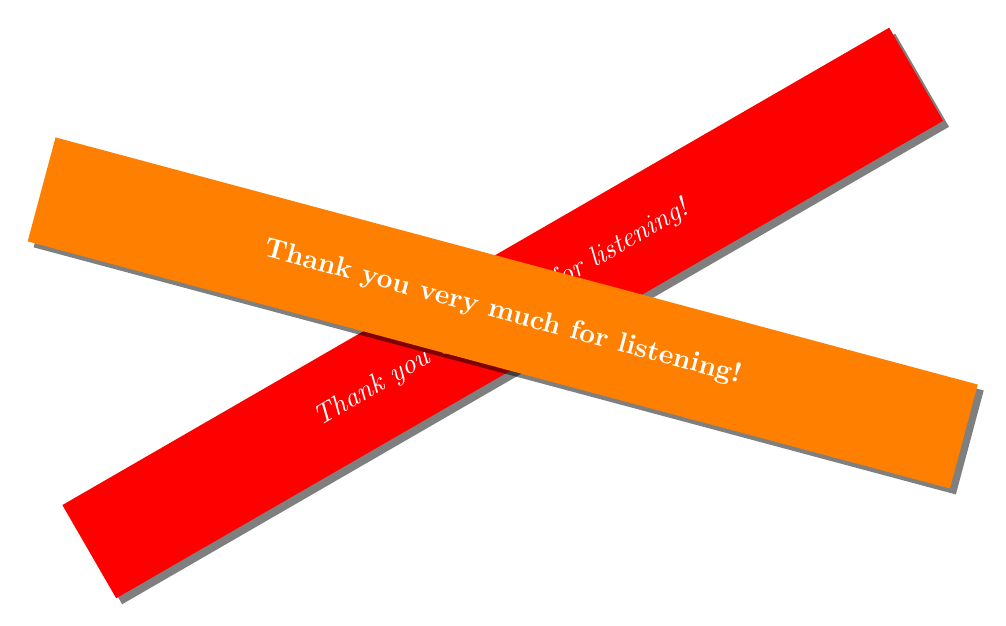
\begin{tikzpicture}[every node/.style={rectangle,inner sep=15pt,minimum width=\textwidth,text=white,drop shadow=black}]
\node[fill=red,rotate=30] {\ita{Thank you very much for listening!}};
\node[fill=orange,rotate=-15] {\fat{Thank you very much for listening!}};
% \node[fill=red,rotate=30] {\fat{Thank you very much for listening!}};
% \node[fill=orange,rotate=15] {\fat{Thank you very much for listening!}};
% \node[fill=green,rotate=0] {\fat{Thank you very much for listening!}};
% \node[fill=blue,rotate=-15] {\fat{Thank you very much for listening!}};
% \node[fill=red,rotate=-30] {\fat{Thank you very much for listening!}};
\end{tikzpicture}
\end{frame}

% Following frames are counted separately with the appendixnumberbeamer package
\appendix
%------------------------------------------------------------------------------%
% References
%------------------------------------------------------------------------------%
\begin{frame}[t,allowframebreaks]{References}
%\nocite{*} % If active, display all bib entries, and not just the cited ones
\bibliographystyle{apalike}
{\tiny
\bibliography{../bib/buchi_compl.bib}}
\end{frame}


\end{document}
